\subsubsection{Reward Interactions}
\nestindent

We analyze interaction effects by comparing combined runs to their constituent individual rewards.

\textbf{A+B: Mild interference.}
The A+B run (\pFourCombinedAbDeltaPassOne{}pp) underperforms the best individual component A (\pFourSeparateADeltaPassOne{}pp) by 0.4pp.
This mild interference may stem from the proximity reward (B) providing noisy gradient that dilutes the format reward's cleaner signal.
Notably, A+B's sequence length follows the baseline's declining trend rather than A's increasing trend, suggesting B's signal dominates the length dynamics.

\textbf{C+D: Additive on Pass@1, synergistic on Pass@8.}
C+D (\pFourCombinedCdPassOne\% Pass@1) approximately equals C alone (\pFourSeparateCPassOne\%), indicating no Pass@1 synergy.
However, C+D achieves higher Pass@8 (\pFourCombinedCdPassEight\% vs.\ C's \pFourSeparateCPassEight\%), suggesting D contributes diversity of correct solutions.
The extraction failure rate improves further (\pFourCombinedCdExtrFail\% vs.\ C's \pFourSeparateCExtrFail\%).

\textbf{C+D+E: Best knowledge ceiling.}
Adding number grounding to C+D yields the highest Pass@8 of any configuration (\pFourCombinedCdePassEight\%) and the lowest extraction failure rate (\pFourCombinedCdeExtrFail\%).
However, Pass@1 (\pFourCombinedCdePassOne\%) is lower than E alone (\pFourSeparateEPassOne\%), suggesting that the three grounding rewards together create a conservative policy that solves more problems but less reliably on the first attempt.
The \pFourCombinedCdeGap{}pp Pass@8--Pass@1 gap (the widest of any run) supports this interpretation.
Zero gibberish responses and only \pFourCombinedCdeNoAnswer\% ``no answer'' failures confirm that C+D+E nearly eliminates surface-level degeneration.

\textbf{Comb.\ All: Constructive composition.}
The Comb.\ All run (\pFourCombinedAllPassOne\% Pass@1, \pFourCombinedAllDeltaPassOne{}pp) substantially exceeds any individual reward or pair.
For comparison, the sum of individual improvements is A(\pFourSeparateADeltaPassOne) + B(\pFourSeparateBDeltaPassOne) + C(\pFourSeparateCDeltaPassOne) + D(\pFourSeparateDDeltaPassOne) + E(\pFourSeparateEDeltaPassOne) = +12.6pp, while the actual combined improvement is \pFourCombinedAllDeltaPassOne{}pp.
This sub-additivity is expected: the rewards target overlapping failure populations, so their effects are partially redundant.
However, the Comb.\ All run gains \pFourCombinedAllGained{} problems (more than any individual) while losing only \pFourCombinedAllLost, indicating that the rewards access complementary subsets of solvable problems.

\textbf{Loss stability.}
A striking pattern across all ten configurations: the number of lost problems (relative to baseline) is remarkably stable at \pFourLossMin--\pFourLossMax, regardless of which or how many rewards are used.
This suggests a fixed population of $\sim$50 problems that become harder under any reward perturbation---possibly problems whose solutions depend on behaviors that additional reward signals disrupt.
The gains, by contrast, scale with reward count (individual: 55--98, pairs: 77--96, triples: 96, full: \pFourCombinedAllGained), driving net improvement.

Figure~\ref{fig:p4-interactions} visualizes the interaction patterns: panel~(a) compares the expected improvement (sum of individual $\Delta$Pass@1 values) against the actual combined improvement, revealing consistent sub-additivity; panel~(b) compares each combined run to its best individual component on both Pass@1 and Pass@8, revealing that grounding combinations (C+D, C+D+E) trade first-attempt reliability for knowledge ceiling.

\vspace{1em}
\noindent\begin{minipage}{\linewidth}
\centering
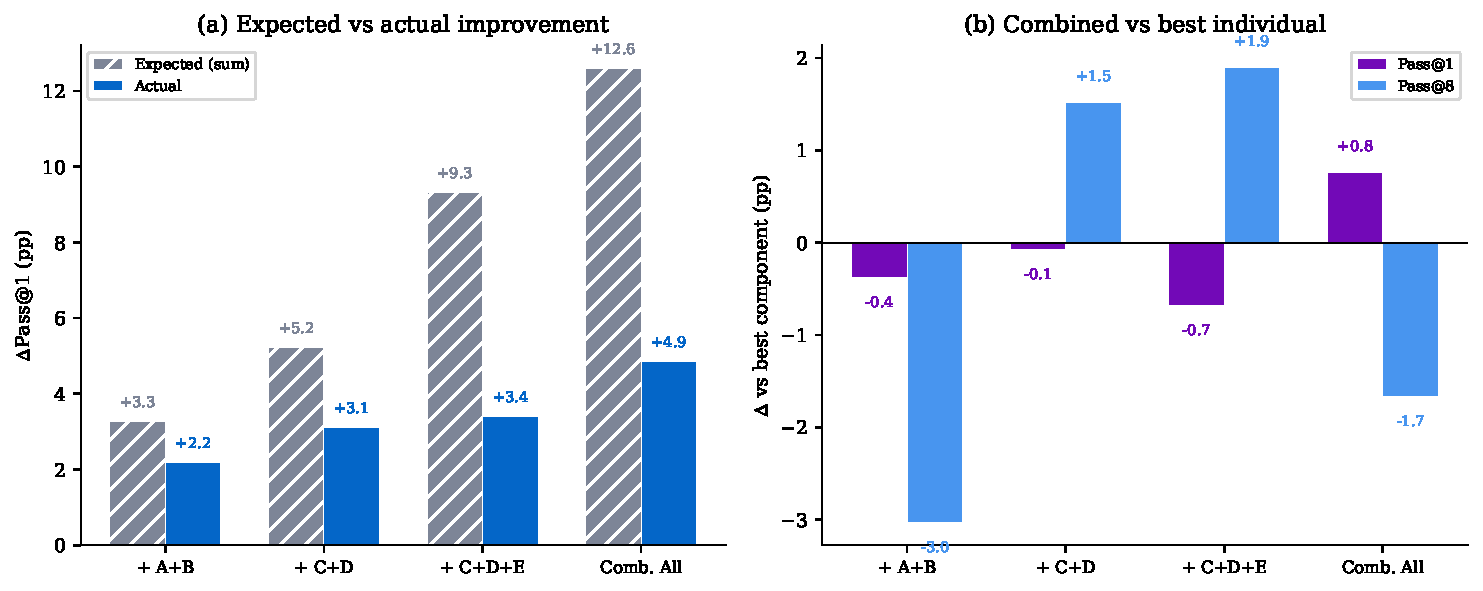
\includegraphics[width=\linewidth]{component/figures/p4/fig3_interactions.pdf}
\captionof{figure}{Reward interaction patterns. (a)~Expected (sum of components) vs.\ actual $\Delta$Pass@1 for each combined run. (b)~$\Delta$ vs.\ best individual component on Pass@1 and Pass@8.}
\label{fig:p4-interactions}
\end{minipage}
\vspace{1em}
\nestunindent
